
\medskip 

\parbox{0.45\linewidth}{Chaque été, Jean exploite son marais salant sur l'île de Ré, situé dans l'océan Atlantique, près de La Rochelle.}\hfill
\parbox{0.45\linewidth}{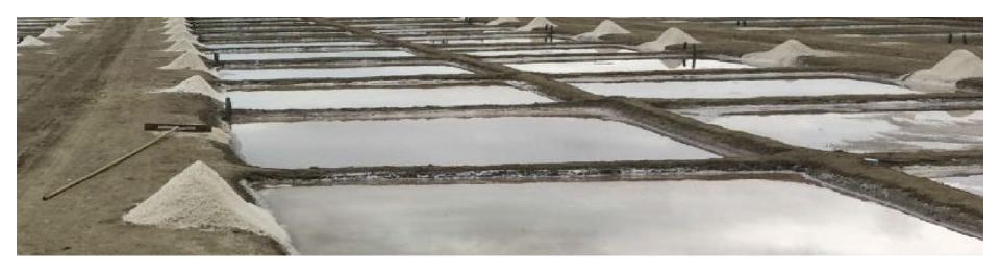
\includegraphics[width=5.5cm]{marais_salant}}

\medskip

Son marais se compose de carreaux (carrés de 4 m de côté) dans lesquels se récolte le sel.

\bigskip

\textbf{Partie A. Le gros sel}

\medskip

Chaque jour, il récolte du gros sel sur 25 carreaux. Le premier jour, afin de prévoir sa production, il relève la masse en kilogramme de chaque tas de gros sel produit par carreau.

Voici la série statistique obtenue :

\[34~;~39 ~;~  31 ~;~  45 ~;~  40 ~;~  32 ~;~  36 ~;~  45 ~;~  42 ~;~  34 ~;~  30 ~;~  48 ~;~  43~;~
32 ~;~  39 ~;~  40 ~;~ 42 ~;~  38 ~;~  46 ~;~  31 ~;~  38 ~;~  43 ~;~  37 ~;~  47 ~;~  33\]

\medskip

\begin{enumerate}
\item Calculer l'étendue de cette série statistique.
\item Déterminer la médiane de cette série statistique et interpréter le résultat.
\item Calculer la masse moyenne en kg des tas de gros sel pour ce premier jour.
\end{enumerate}

\bigskip

\textbf{Partie B. La fleur de sel}

\medskip

La fleur de sel est la mince couche de cristaux blancs qui se forme et affleure la surface des
marais salants. Chaque soir, Jean cueille la fleur de sel à la surface des carreaux. Pour
transporter sa récolte, il utilise une brouette comme sur le schéma ci-dessous.

\begin{center}
\psset{unit=0.75cm}
\begin{pspicture}(18,6.5)
%\psgrid
\pspolygon(0.9,4.7)(6,4.7)(7.1,5.4)(2,5.4)
\psline(0.9,4.7)(2.9,2.2)(6,2.2)(6,4.7)
\psline(6,2.2)(7.1,2.9)
\psline[linestyle=dashed](2.9,2.2)(3.9,2.9)(7.1,2.9)
\psline[linestyle=dashed](3.9,2.9)(2,5.4)
\psline{<->}(5.9,2.2)(5.9,4.7) \uput[l]{90}(5.9,3.45){\small 35 cm}
\pscircle(2.2,1.25){0.15}\pscircle(2.2,1.25){0.3}\pscircle(2.2,1.25){0.66}
\psline(2.9,2.2)(2.17,1.27)\psline(2.22,1.25)(3.4,2.2)
\psline(7.1,2.9)(7.1,5.4)
\psline{<->}(2.9,2)(6,2)\uput[d](4.45,2){40 cm}
\psline{<->}(2,5.6)(7.1,5.6)
\uput[u](4.55,5.6){70 cm}
\psline{<->}(0.7,4.7)(1.7,5.4)\uput[l](1.4,5.25){40 cm}
\psline(5.2,2.2)(5.4,0.4)(5.6,0.4)(6,2.2)
\psline(5.6,0.4)(5.75,0.55)(6.2,2.3)
\psline(6.3,2.45)(6.5,1)(6.7,1)(7,2.82)
\psline(6.7,1)(6.9,1.15)(7.1,2.9)
\psframe(6.9,5.3)(10.4,5.15)
\psline(7.1,5.4)(10.5,5.4)(10.5,5.3)(10.4,5.15)
\psline(10.5,5.4)(10.4,5.3)
\psframe(6,4.7)(9.5,4.55)
\psline(6.2,4.8)(9.6,4.8)(9.6,4.7)(9.5,4.55)
\psline(9.6,4.8)(9.5,4.7)
\pspolygon(9,3.4)(11,3.4)(12,2)(7.5,2)
\psline[linestyle=dashed](11,3.4)(11,2)\psframe(11,2.2)(10.8,2)
\uput[l](11,2.7){$h$}
\uput[u](10,3.4){$b$} \uput[d](9.75,2){$B$}
\rput(10.4,4.1){Trapèze}\uput[l](11,2.7){$h$}
\rput(9.75,0.7){Aire $ = \dfrac{(B + b) \times h}{2}$}
\pspolygon(13,5)(16.5,5)(15.75,3.5)(14.5,3.5)
\pspolygon[fillstyle=solid,fillcolor=lightgray](13,2)(16.5,2)(15.75,0.5)(14.5,0.5)
\psline(13,5)(13,2)\psline(16.5,5)(16.5,2)\psline(15.75,0.5)(15.75,3.5)\psline(14.5,3.5)(14.5,0.5)
\rput(15,1.25){Aire base}\uput[r](16.5,3.5){hauteur}
\rput(14.5,6.){Prisme droit}
\rput(14.75,0.2){Volume = Aire base $\times$ hauteur}
\end{pspicture}
\end{center}

\medskip

\begin{enumerate}
\item Montrer que cette brouette a un volume de 77 litres.
\item Sachant que 1 litre de fleur de sel pèse $900$ grammes, calculer la masse en kg du contenu d'une brouette remplie de fleur de sel.
\end{enumerate}

\vspace{0.5cm}

